%
\section{Findings}
%
Due to the subjective nature of estimating the overall quality of our video summaries we test our results on a panel of test users. We use various methods to generate the summaries and present them to this panel for review.
%
\subsection{Test Environment}
%
Our test environment is a website showing a collection of generated videos, hosted on YouTube. Visitors are shown one video at a time, and are presented with a questionnaraire after the video is done playing.
%
\subsubsection{Questionnaire}
%
% reverse engineer questions (find lit. on how to write a questionnaire)
%
The questionnaire for each video consists of four statements to which the user can \textit{disagree}, \textit{somewhat disagree}, \textit{somewhat agree}, \textit{agree} or declare that she \textit{does not know}. In an attempt to discourage the user from selecting the latter option it is shown last in the list. Based on feedback from an initial, single-user test run we also added and introduction page that explains the purpose of the test and shows the available statements and options. The description is also present throughout the test.\\
%
The four statements shown after each video are:
%
\begin{itemize}
\item The individual video clips are interesting
\item The video is well edited
\item The length of the individual video clips are fitting
\item The length of the entire video is fitting
\end{itemize}
%
The first statement investigates the quality of our choice of labels, and to some degree also the quality of our classifiers. The second statement investigates how well we are able to combine segments (in other words the quality of our recipe, ie. the order and context of the ingredients). The third statement investigates the general attitude towards clip-length, which is chosen somewhat at random within boundaries determined by the recipe. The fourth statement investigates the general attitude towards the total length of a video-summary. We also added an optional note to each questionnaire in case a user wanted to ellaborate on her answer(s).
%
\subsubsection{Setup}
%
Our test environment runs on \textit{Google App Engine} and consist of a minimalistic website. To discern interuptive elementsplayer-controls are removed from the YouTube embedded player (the user can still pause the video by clicking on it or by using the space-bar on their keyboard). The questionnaire was not shown before the end of the video in order not to disctract attention to it. The video-title, which would appear briefly in the top of the player is the hex-value of a randomly generated number to ensure a non-descript title.\\
Each user session is tracked using a randomly generated identifier. We do not make any attempt to track users across different sessions so we are unable to track a returning test-user, but it does give us a rough measure of how many different test-users we have, how many questionnaires they answered on average.\\
To increase the availability of our test environment everything is localised into danish and english. The resulting locale is recorded along with each result, in case the specific translations have an effect on our results. All text in the test is available in Appendix [SEC:REF], in both languages.\\
The test is designed so that the test user can see as few or as many videos as she wants. A circular queue of videos is shared between all users, meaning that a new user will start at the video following the one that was last rated. Answers are stored after each succesful rating.\\
The test users concist of friends and relatives contacted through facebook. In order to help spread the test to more people we also placed a Facebook Like-button and a Twitter button discretely in the bottom of the questionnaires.\\\\
%
The test website can be found at http://thesis.fmitcar.appspot.com/thesis/start/
%
\subsection{Test videos}
%
We investigate several aspects of the video summary aggregation. Most importantly we investigate how our automatically generated video summaries compare to human edited ones, and how both these groups compare to randomly generated video summaries.
%
\subsubsection{Random}
%
\textit{Random} video summaries are generated without any use of labels. They consist of 6 videclips selected randomly from the footage for a particular event. Each clip has a random length between 2 and 10 seconds. Only one clip is selected from each video, in order to avoid repeating or overlapping footage, which would be a dead giveaway. These video summaries are thought of as a baseline - we expect them to perform poorly.
%
\subsubsection{Random label}
%
These video summaries are slightly \textit{less} random. Instead of selecting video clips randomly from the footage, we instead generate a random recipe and create a video summary from it. This is done by generating a sequence of 5 \textit{ingredients} (described in section [SEC:REF]), each containing a random set of 1 to 3 \textit{requested labels}. The minimum length of a video clip, $min$, is set to be somewhere between 2 and 9 seconds. The maximum length is set to be somewhere between $min$ and $2 \cdot min$.\\
Because these video summaries are based on footage where labels were detected, we expect their content to be of higher quality than the videos described in the previous section.
%
\subsubsection{Designer}
%
The \textit{designer} video summaries are based on our own recipe.
We designed a recipe to be used on all three datasets. Ingredients outlined below:
\begin{itemize}
\item Overview shot, 3-5 seconds, no person in focus
\item Overview shot, 3-6 seconds, no person in focus
\item Crowd shot, 3-6 seconds, no person in focus
\item Crowd shot, 3-6 seconds, no person in focus
\item Person in focus shot, 4-8 seconds, not in a crowd
\item Person in focus shot, 4-8 seconds, not in a crowd
\item Overview shot, 3-5 seconds, no person in focus
\end{itemize}
%
During recipe tweaking we realized that the overview label and person in focus label often overlapped. To reduce the odds of having a person in focus on overview shots we put this label into the forbidden labels list (an overview can still have a person in focus not caught by our labeller).\\
Likewise there are typically two types of crowd shots. One has someone in focus, and the other one has not. We wanted the last type.
%
\subsubsection{Human edited}
%
We used human edited videoclips as a control sample. A select few videos was cut to fit the general length of other computer generated videoclips. We expect these to perform as well as the designer recipies or better.
%
\subsubsection{Other aspects}
%
% datasets, alpha span
%
\subsubsection{Table}
%
INSERT TABLE HERE!!!
%
\subsection{Results}
%
INTRO
%
\subsubsection{Feedbackme}
%
% OVERVIEW OVER ANSWERS (TABLE) #ANSWERS, #SESSIONS, #ANSWERS/SESSION, ETC. 
%
\subsubsection{Histograms}\label{sec:histograms}
%
% ANDERS
Histograms shows the distribution of data, and is a visual tool to aid in determining if data follows a specific probability distribution. We have divided our histograms into 5 bins, where each bin corresponds to a specific answer to our questionnaire. Each bin is thus, from left to right, Totally Disagree, Somewhat Disagree, Don't Know, Somewhat Agree, Totally Agree.
% \newpage
%
\begin{figure}[h!]
     \centering
     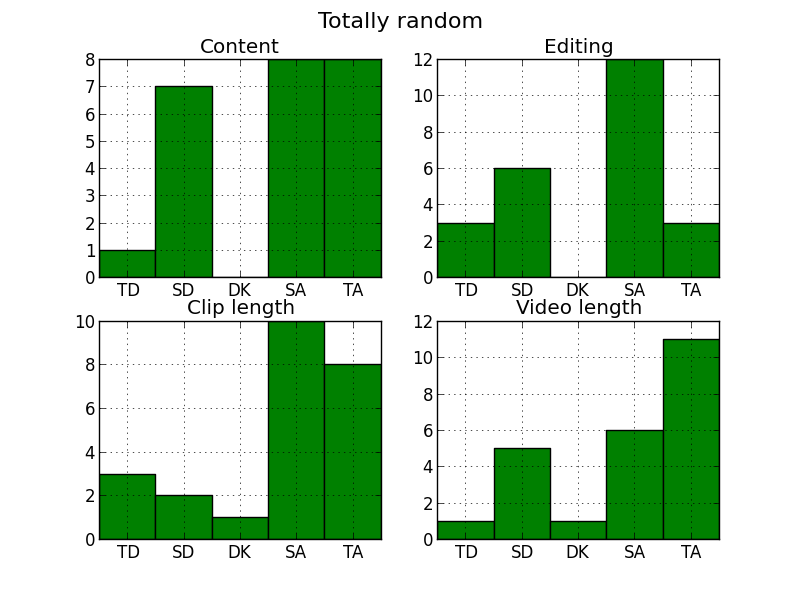
\includegraphics[width=0.7\textwidth]{img/totallyrandom_barplot.png}
     \caption{Histogram of answers to videos created using random segments}\label{fig:hist_random}
\end{figure}
%
\begin{figure}[h!]
     \centering
     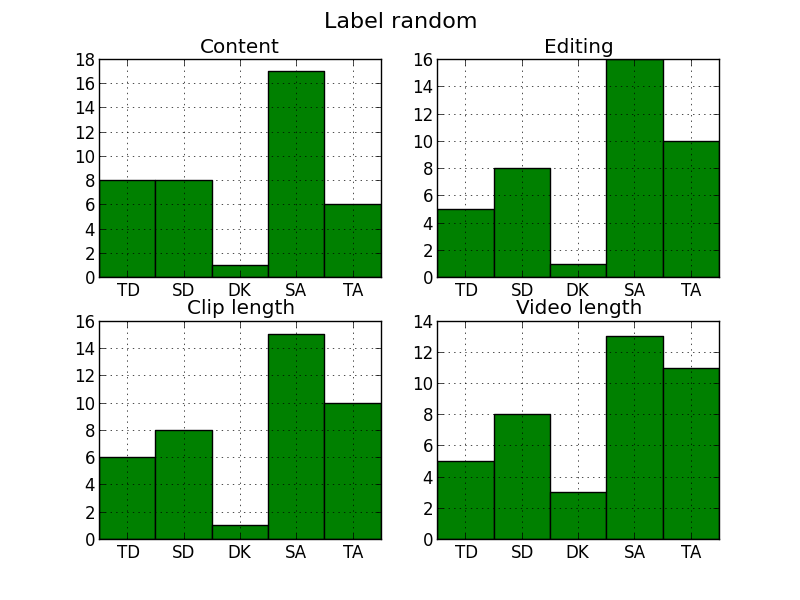
\includegraphics[width=0.7\textwidth]{img/labelrandom_barplot.png}
     \caption{Histogram of answers to videos created using the random label recipe}\label{fig:hist_labelrandom}
\end{figure}
% \newpage
%
\begin{figure}[h!]
     \centering
     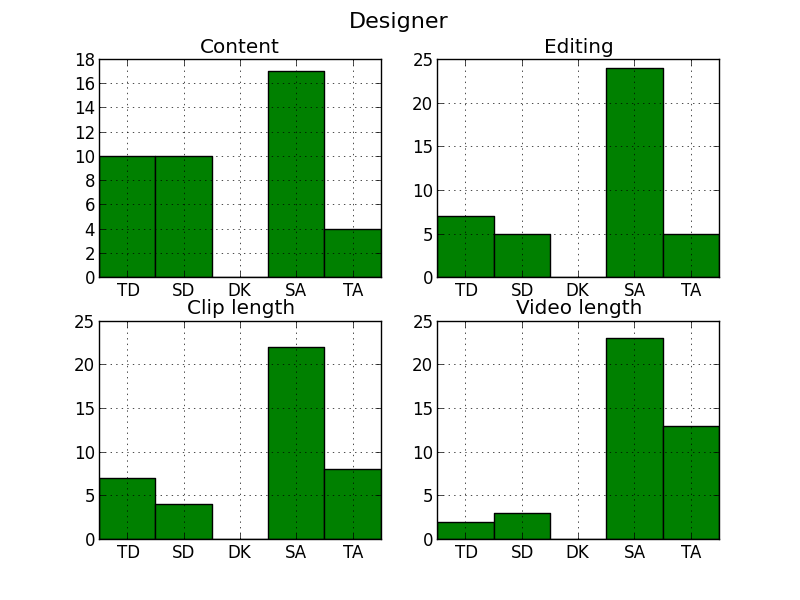
\includegraphics[width=0.7\textwidth]{img/designer_barplot.png}
     \caption{Histogram of answers to videos created using the designer method}\label{fig:hist_design}
\end{figure}
%
\begin{figure}[h!]
     \centering
     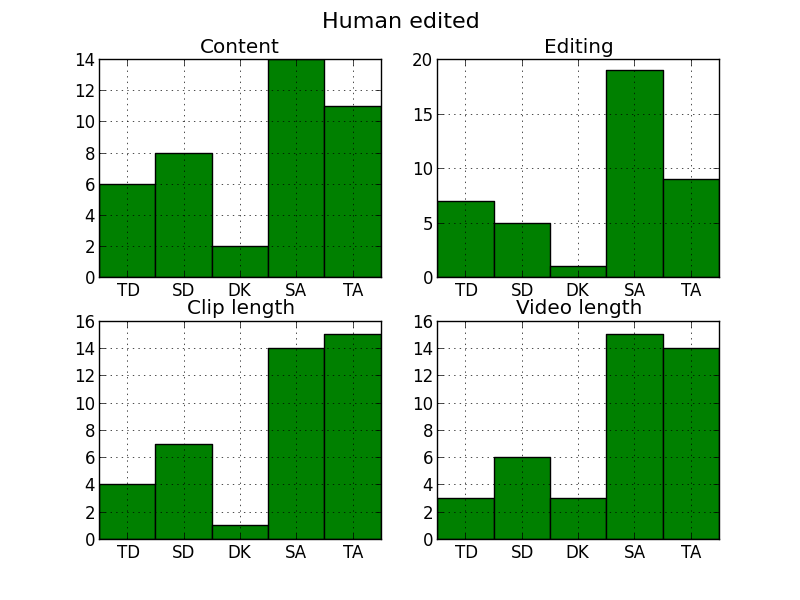
\includegraphics[width=0.7\textwidth]{img/humanedited_barplot.png}
     \caption{Histogram of answers to videos that are edited by a human}\label{fig:hist_human}
\end{figure}
%
\subsubsection{Friedman Test}
%
The Friedman rank sum test is a non-parametric statistical test, and is used to detect differences in methods in multiple tests. In our case we have multiple methods as described in section \ref{sec:}, and each test participant can be viewed as a seperate test. We test against the null-hypothesis which in a general form is that there is no significant measureable difference in the methods applied to generate a video.\\
%
The histograms in section \ref{sec:histograms} shows us that the data does not follow any specific distribution, which forces us to deploy a non-parametric statistical test. The disadvantage of employing a non-parametric test is that it requires are larger sample size to draw conclusions with the same degree of confidence as a parametric test.\\
%
The values related to each answer are also not compareable (there is no clear numerical interpretation), ie. \textit{Totally Disagree} $(-2)$ is not twice as bad as \textit{Somewhat Disagree} $(-1)$, but \textit{Totally disagree} is ranked lower than \textit{Somewhat disagree}. The Friedman test ranks all answers, where answers with equal values receive the same rank, and then sums occurences of each rank.\\
%
Results of our Friedman test can be found in Tables \ref{tab:fried_alpha}, \ref{tab:fried_dataset}, and \ref{tab:fried_recip} where $\nu$ denotes degrees of freedom, and p-value is \textit{"the probability of obtaining a test statistic at least as extreme as the one that was actually observed, assuming that the null hypothesis is true."}\footnote{http://en.wikipedia.org/wiki/P-value}. A p-value less than $0.05$ is considered statistically significant.
% INPUT IS 3 TABLES
\begin{table}[ht]
	\begin{center}
	\caption{Friedman rank sum test for recipies}
	\label{tab:fried_recip}
		\begin{tabular}{lccc}
		\toprule
			 & v & p-value & $x^2$\\
			\midrule
			Content & $3$ & $0.3242$ & $3.4737$\\
			Editing & $3$ & $0.3260$ & $3.4602$\\
			Clip length & $3$ & $0.9597$ & $0.3016$\\
			Video length & $3$ & $0.3218$ & $3.4918$\\
			Total score & $3$ & $0.4882$ & $2.4292$\\
		\bottomrule
		\end{tabular}
	\end{center}
\end{table}
\begin{table}[ht]
	\begin{center}
	\caption{Friedman rank sum test for datasets}
	\label{tab:fried_dataset}
		\begin{tabular}{lccc}
		\toprule
			 & v & p-value & $x^2$\\
			\midrule
			Content & $2$ & $0.0773$ & $5.1193$\\
			Editing & $2$ & $0.5436$ & $1.2190$\\
			Clip length & $2$ & $0.0577$ & $5.7059$\\
			Video length & $2$ & $0.2030$ & $3.1887$\\
			Total score & $2$ & $0.1185$ & $4.2656$\\
		\bottomrule
		\end{tabular}
	\end{center}
\end{table}
\begin{table}[ht]
	\begin{center}
	\caption{Friedman rank sum test for $\alpha$-span}
	\label{tab:fried_alpha}
		\begin{tabular}{lccc}
		\toprule
			 & v & p-value & $x^2$\\
			\midrule
			Content & $1$ & $0.7055$ & $0.1429$\\
			Editing & $1$ & $1.0000$ & $0.0000$\\
			Clip length & $1$ & $0.4652$ & $0.5333$\\
			Video length & $1$ & $0.7055$ & $0.1429$\\
			Total score & $1$ & $0.5271$ & $0.4000$\\
		\bottomrule
		\end{tabular}
	\end{center}
\end{table}
%
\\ %newline after input table
Table \ref{tab:fried_recip} shows the result from videos generated by the each method, Table \ref{tab:fried_dataset} shows the results from videos partitioned by which dataset a given video is generated from, and Table \ref{tab:fried_alpha} shows the effect of different $\alpha$-span values (described in section \ref{sec:})
%
\subsubsection{Notes}
%
% ANDERS
PRESENT QUEST. NOTES (need to extract these first)
%
\subsection{Analysis}
%
ANALYSIS OF NOTES, ?\\
Figure \ref{fig:hist_random} and \ref{fig:hist_human} shows that answers are unevenly distributed with a skew to the right, ie. answers generally agrees with the statements. Figure \ref{fig:hist_labelrandom} shows that answers are somewhat evenly distributed, not counting the Don't Know answer. There is no discernable consent with the statement. Figure \ref{fig:hist_design} shows that answers are unevenly distributed with a skew to the right with the exception of the "content" statement.\\
The only statistical significance is \textit{content} in Table \ref{tab:fried_dataset}. As everything else is statistically insignificant we do not pursue further statistical analysis.
As we are unable to reject the null hypothesis in almost all regards we conclude that the questionaires reveal no significant effect of the various methods of generating a the resulting video. This also means that there is no significant measureable difference between a human edited video and one that is generated at random.\\
There is also no significant measureable effect of choosing different $\alpha$-values, ref to section with alpha-values explained. We only tested for two different values to keep the number of test videos at a manageable level.\\
There was also no significant measureable difference between the three datasets, except in content which is no surprise as the datasets differ primarily on content as described in section \ref{section that describes datasets}.\\
%
\subsection{Risks \& Limitations}
%
User based tests are inherently risky. Our choice of statements and options are bound to have had a huge influence on the results. As is the choice of supporting two languages. Based on feedback from users (both through the test and in person) we have come to understand that several things could have been done better. Several users complained over the lack of context in which they were watching the video. They claimed, rightfully, that it is almost impossible to determine whether clips were interresting or whether the length of a video is fitting, when they did not know what they were watching. The lack of sound only makes this more difficult.\\\\
%
Lots more here...
% LAUGE
% limited dataset -> we did not have seperate training and test sets\\     <- Skal stå i forrige sektion
% barely acceptable amount of feedback -> could have caused ...
% search keywrod kunne måske have hjulpet på at forstå spøgsmål bedre.
%
\section{Summary}
%
% LAUGE

%
% ANDERS

%
We believe that this is an effect of high quality raw material, and we would suspect that there would be a noticeable difference if our dataset had contained a larger amount of video footage of questionable quality; visual, contextual, or both.\\
which leads us to conclude that we must test for values closer to the extreme to get a definite answer. FURTHER ANALYSIS COULD BE TO INVESTIGATE THE EFFECT OF ALPHA VALUES, IE. FOR ALPHA VALUE X WE GET A TOTAL AVR. VIDEO LENGTH OF SO AND SO SECONDS, AND SEGMENT LENGTHS OF SO AND SO SECONDS, COMPARE THAT TO AN ALPHA VALUE OF 2X.\\
%